% Proposta G (12/11/2026, pedido do autor): a B, que o autor achou a melhor, mais
% simples e mais intuitiva. Duas faixas lado a lado, uma por pergunta ("Direção:
% para que lado?" e "Risco: com que risco?"). As duas nascem do mesmo ARIMA e se
% juntam embaixo na ordem, que é a integração. O losango fica na faixa do risco e
% só recebe a volatilidade (o filtro só olha a volatilidade). Sem fórmula: o
% ajuste da posição diz só "maior volatilidade, posição menor". Mesmo estilo das
% fig05/fig06. Fora do TG até o autor decidir.
\documentclass[11pt,border=2pt]{standalone}
\usepackage[T1]{fontenc}
\usepackage[utf8]{inputenc}
\usepackage{mathptmx}
\usepackage{tikz}
\usetikzlibrary{arrows.meta,positioning,calc,shapes.geometric,fit,backgrounds}
\tikzset{
  seta/.style={-{Stealth[length=2.2mm]}, semithick},
  caixa/.style={rectangle, draw, semithick, fill=gray!10, rounded corners=2pt,
                align=center, minimum width=44mm, minimum height=10mm, font=\small},
  dado/.style={trapezium, trapezium left angle=75, trapezium right angle=105, draw,
               semithick, fill=white, align=center, minimum height=9mm, font=\small,
               trapezium stretches body},
  decisao/.style={diamond, draw, semithick, fill=white, aspect=2.4, align=center,
                  inner sep=1pt, font=\small},
  faixa/.style={rectangle, draw=gray!55, fill=gray!4, rounded corners=4pt, inner sep=3mm},
  titulo/.style={font=\small, align=left, anchor=north west},
  pequeno/.style={font=\footnotesize},
}
\begin{document}
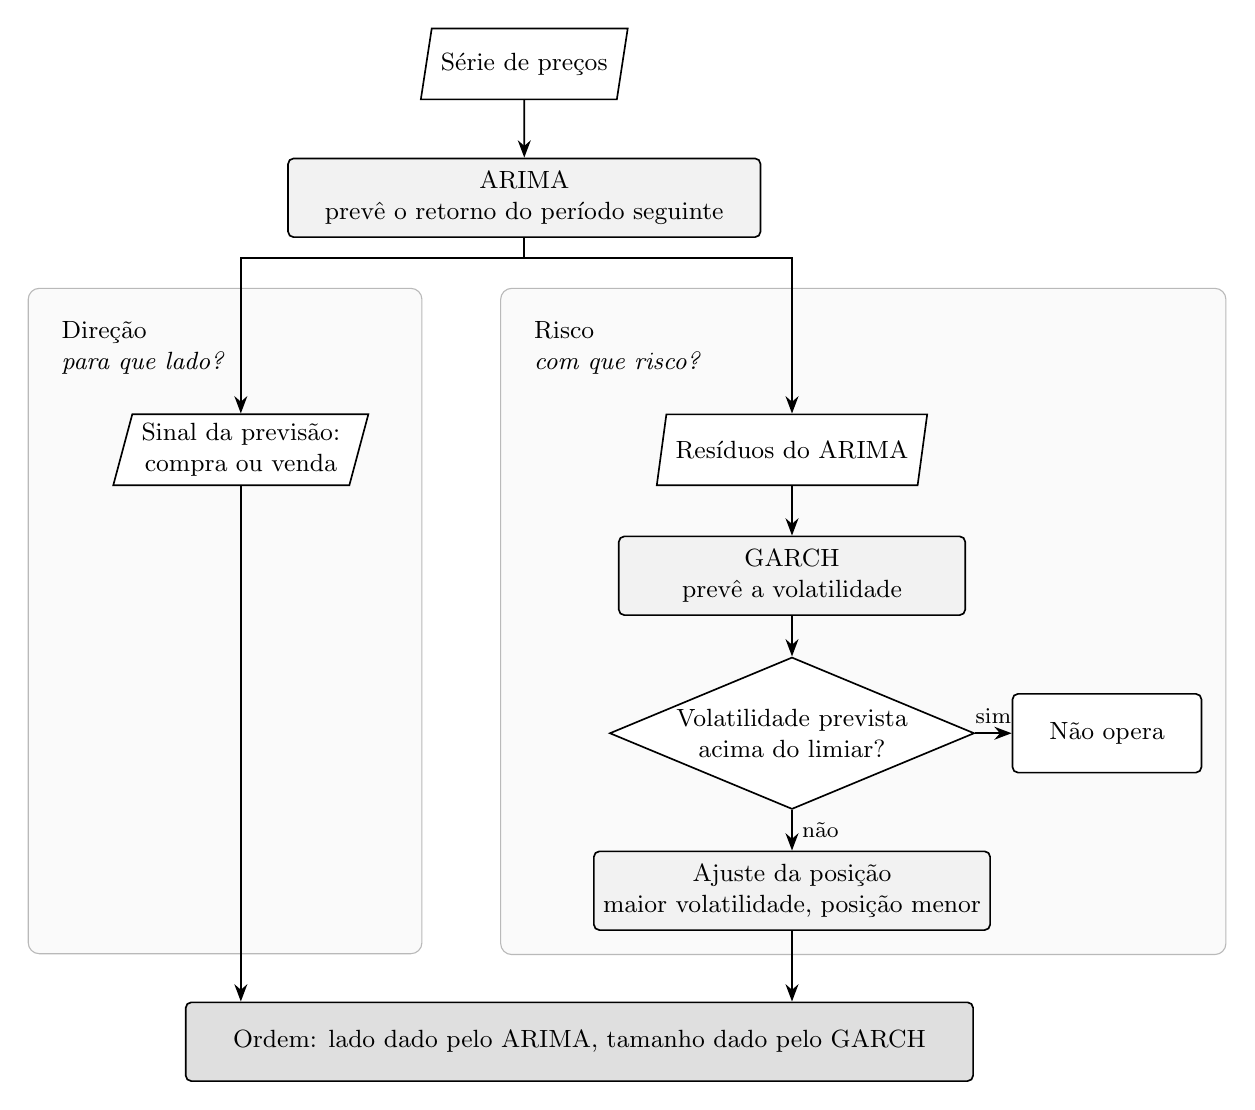
\begin{tikzpicture}
  \node[dado] (ent) at (0,0) {Série de preços};
  \node[caixa, minimum width=60mm] (arima) at (0,-1.7) {ARIMA\\prevê o retorno do período seguinte};

  % faixa da direção
  \node[titulo] (td) at (-6.0,-3.15) {Direção\\\textit{para que lado?}};
  \node[dado] (dir) at (-3.6,-4.9) {Sinal da previsão:\\compra ou venda};
  \coordinate (fd) at (-1.6,-11.0);

  % faixa do risco
  \node[titulo] (tr) at (0.0,-3.15) {Risco\\\textit{com que risco?}};
  \node[dado] (res) at (3.4,-4.9) {Resíduos do ARIMA};
  \node[caixa] (garch) at (3.4,-6.5) {GARCH\\prevê a volatilidade};
  \node[decisao] (lim) at (3.4,-8.5) {Volatilidade prevista\\acima do limiar?};
  \node[caixa, minimum width=24mm, fill=white] (veto) at (7.4,-8.5) {Não opera};
  \node[caixa] (tam) at (3.4,-10.5) {Ajuste da posição\\maior volatilidade, posição menor};

  \begin{scope}[on background layer]
    \node[faixa, fit=(td) (dir) (fd)] (fdir) {};
    \node[faixa, fit=(tr) (res) (garch) (lim) (veto) (tam)] (frisco) {};
  \end{scope}

  % a integração: as duas faixas se juntam na ordem
  \path (fdir.south) ++(0,-6mm) coordinate (base);
  \node[caixa, fill=gray!25, minimum width=100mm, anchor=north] (ord) at (base -| 0.7,0) {Ordem: lado dado pelo ARIMA, tamanho dado pelo GARCH};

  \draw[seta] (ent) -- (arima);
  \draw[seta] (arima.south) -- ++(0,-0.25) -| (dir.north);
  \draw[seta] (arima.south) -- ++(0,-0.25) -| (res.north);
  \draw[seta] (res) -- (garch);
  \draw[seta] (garch) -- (lim);
  \draw[seta] (lim) -- node[above, pequeno]{sim} (veto);
  \draw[seta] (lim) -- node[right, pequeno]{não} (tam);
  \draw[seta] (tam.south) -- (tam.south |- ord.north);
  \draw[seta] (dir.south) -- (dir.south |- ord.north);
\end{tikzpicture}
\end{document}
